       \documentclass[journal, a4paper]{IEEEtran}

% some very useful LaTeX packages include:

%\usepackage{cite}      % Written by Donald Arseneau
                        % V1.6 and later of IEEEtran pre-defines the format
                        % of the cite.sty package \cite{} output to follow
                        % that of IEEE. Loading the cite package will
                        % result in citation numbers being automatically
                        % sorted and properly "ranged". i.e.,
                        % [1], [9], [2], [7], [5], [6]
                        % (without using cite.sty)
                        % will become:
                        % [1], [2], [5]--[7], [9] (using cite.sty)
                        % cite.sty's \cite will automatically add leading
                        % space, if needed. Use cite.sty's noadjust option
                        % (cite.sty V3.8 and later) if you want to turn this
                        % off. cite.sty is already installed on most LaTeX
                        % systems. The latest version can be obtained at:
                        % http://www.ctan.org/tex-archive/macros/latex/contrib/supported/cite/
 \usepackage{algorithm}
\usepackage[noend]{algpseudocode}
\makeatletter
\def\BState{\State\hskip-\ALG@thistlm}
\makeatother
\usepackage{amssymb}
\usepackage{graphicx}   % Written by David Carlisle and Sebastian Rahtz
                        % Required if you want graphics, photos, etc.
                        % graphicx.sty is already installed on most LaTeX
                        % systems. The latest version and documentation can
                        % be obtained at:
                        % http://www.ctan.org/tex-archive/macros/latex/required/graphics/
                        % Another good source of documentation is "Using
                        % Imported Graphics in LaTeX2e" by Keith Reckdahl
                        % which can be found as esplatex.ps and epslatex.pdf
                        % at: http://www.ctan.org/tex-archive/info/

%\usepackage{psfrag}    % Written by Craig Barratt, Michael C. Grant,
                        % and David Carlisle
                        % This package allows you to substitute LaTeX
                        % commands for text in imported EPS graphic files.
                        % In this way, LaTeX symbols can be placed into
                        % graphics that have been generated by other
                        % applications. You must use latex->dvips->ps2pdf
                        % workflow (not direct pdf output from pdflatex) if
                        % you wish to use this capability because it works
                        % via some PostScript tricks. Alternatively, the
                        % graphics could be processed as separate files via
                        % psfrag and dvips, then converted to PDF for
                        % inclusion in the main file which uses pdflatex.
                        % Docs are in "The PSfrag System" by Michael C. Grant
                        % and David Carlisle. There is also some information
                        % about using psfrag in "Using Imported Graphics in
                        % LaTeX2e" by Keith Reckdahl which documents the
                        % graphicx package (see above). The psfrag package
                        % and documentation can be obtained at:
                        % http://www.ctan.org/tex-archive/macros/latex/contrib/supported/psfrag/

%\usepackage{subfigure} % Written by Steven Douglas Cochran
                        % This package makes it easy to put subfigures
                        % in your figures. i.e., "figure 1a and 1b"
                        % Docs are in "Using Imported Graphics in LaTeX2e"
                        % by Keith Reckdahl which also documents the graphicx
                        % package (see above). subfigure.sty is already
                        % installed on most LaTeX systems. The latest version
                        % and documentation can be obtained at:
                        % http://www.ctan.org/tex-archive/macros/latex/contrib/supported/subfigure/

\usepackage{url}        % Written by Donald Arseneau
                        % Provides better support for handling and breaking
                        % URLs. url.sty is already installed on most LaTeX
                        % systems. The latest version can be obtained at:
                        % http://www.ctan.org/tex-archive/macros/latex/contrib/other/misc/
                        % Read the url.sty source comments for usage information.

%\usepackage{stfloats}  % Written by Sigitas Tolusis
                        % Gives LaTeX2e the ability to do double column
                        % floats at the bottom of the page as well as the top.
                        % (e.g., "\begin{figure*}[!b]" is not normally
                        % possible in LaTeX2e). This is an invasive package
                        % which rewrites many portions of the LaTeX2e output
                        % routines. It may not work with other packages that
                        % modify the LaTeX2e output routine and/or with other
                        % versions of LaTeX. The latest version and
                        % documentation can be obtained at:
                        % http://www.ctan.org/tex-archive/macros/latex/contrib/supported/sttools/
                        % Documentation is contained in the stfloats.sty
                        % comments as well as in the presfull.pdf file.
                        % Do not use the stfloats baselinefloat ability as
                        % IEEE does not allow \baselineskip to stretch.
                        % Authors submitting work to the IEEE should note
                        % that IEEE rarely uses double column equations and
                        % that authors should try to avoid such use.
                        % Do not be tempted to use the cuted.sty or
                        % midfloat.sty package (by the same author) as IEEE
                        % does not format its papers in such ways.

\usepackage{amsmath}    % From the American Mathematical Society
                        % A popular package that provides many helpful commands
                        % for dealing with mathematics. Note that the AMSmath
                        % package sets \interdisplaylinepenalty to 10000 thus
                        % preventing page breaks from occurring within multiline
                        % equations. Use:
%\interdisplaylinepenalty=2500
                        % after loading amsmath to restore such page breaks
                        % as IEEEtran.cls normally does. amsmath.sty is already
                        % installed on most LaTeX systems. The latest version
                        % and documentation can be obtained at:
                        % http://www.ctan.org/tex-archive/macros/latex/required/amslatex/math/



% Other popular packages for formatting tables and equations include:

%\usepackage{array}
% Frank Mittelbach's and David Carlisle's array.sty which improves the
% LaTeX2e array and tabular environments to provide better appearances and
% additional user controls. array.sty is already installed on most systems.
% The latest version and documentation can be obtained at:
% http://www.ctan.org/tex-archive/macros/latex/required/tools/

% V1.6 of IEEEtran contains the IEEEeqnarray family of commands that can
% be used to generate multiline equations as well as matrices, tables, etc.

% Also of notable interest:
% Scott Pakin's eqparbox package for creating (automatically sized) equal
% width boxes. Available:
% http://www.ctan.org/tex-archive/macros/latex/contrib/supported/eqparbox/

% *** Do not adjust lengths that control margins, column widths, etc. ***
% *** Do not use packages that alter fonts (such as pslatex).         ***
% There should be no need to do such things with IEEEtran.cls V1.6 and later.


% Your document starts here!
\begin{document}

% Define document title and author
    \title{Generalized Aircraft Collision Avoidance Through Deep Reinforcement Learning }
    \author{ACAS1: Dharmesh Tarapore, Vincent Wahl, Kasim Patel, Shantanu Bobhate
    \\dharmesh@bu.edu, vinwah@bu.edu, kasimp93@bu.edu, sbobhate@bu.edu
    }
    \markboth{Boston University CS 542}{}
    \maketitle

% Write abstract here
\begin{abstract}
    The gradual integration of ADS-B\footnote{ADS-B or automatic dependent surveillance-broadcast enables aircraft to determine its position using satellite navigation, which it then broadcasts periodically. ADS-B can serve as a supplement to secondary radar and is eventually slated to replace it.} into the National Airspace System (NAS) has spurred research into its possible use in collision avoidance systems. While most new systems have shown to be much safer than the existing TCAS II (Traffic Alert and Collision Avoidance System), all of them make comparable assumptions about aircraft capabilities, thus restricting their applicability to highly specific classes of airplanes \cite{nextgen}. In this project, we extend a model derived from one such solution and generalize it to almost all powered aircraft by making conservative initial assumptions about their capabilities and then improving them by extrapolating from state action pairs. This modification allows us to provide a truly comprehensive collision avoidance system that can be used in most powered airplanes.   
\end{abstract}

% Each section begins with a \section{title} command
\section{Introduction}
    % \PARstart{}{} creates a tall first letter for this first paragraph
    \IEEEPARstart{}The federally mandated Traffic Alert and Collision Avoidance System (TCAS II) for transport category aircraft has proven remarkably effective at averting mid-air collisions by providing pilots with timely alerts to resolve imminent threats. However, strong assumptions about aircraft capabilities made in the TCAS II logic prevent it from being used in general aviation, where the risk of a mid-air collision is significantly higher \cite{tcaswhite}.
\\Newer collision avoidance systems handle the complexity induced by the steep variance in airplane dynamics by representing the problem as a Partially Observable Markov Decision Process (POMDP)\cite{pomdporig}. Solving a POMDP for a given state-action pair $(a, s)$ yields an action $a'$ on the basis of a policy, $\pi$, and the corresponding reward, $r$, for choosing that action given the initial state. Each discrete state-action pair, its corresponding action, and reward is then stored in a policy table, which can be used to compare future input state-action pairs and output actions on the basis of a policy $\pi$ that maximizes the expected utility for comparable state-action pairs found in the previously saved policy table. Selecting optimal actions thus requires storing millions of finely tuned policy tables, some of which have an average file size on the order of tens of gigabytes. This poses a serious problem for avionics onboard light aircraft, since budget constraints often restrict hardware memory and processing capabilities. Further, the granularity required to provide precise threat resolution policies grows exponentially as the POMDP learning progresses, eliminating the possibility of an online policy estimator that can refine its policy during actual usage \cite{pomdppolicexpansion}.
\\Previous approaches have focused on evaluating the feasibility of using deep reinforcement learning to develop collision avoidance systems for Unmanned Aerial Systems (UAS) by approximating POMDP score tables \cite{deeprlcas}. Yet, all of the strategies explored so far have made strong assumptions about aircraft performance parameters, thus limiting their applicability to a particular class of aircraft. The approach documented by Julian, for example, makes strong assumptions about an aircraft's permissible turn rates to allow for abrupt maneuvers, which, while pragmatic on an unmanned aerial system, cannot extend to manned aircraft constrained by weight-induced structural limitations and delayed human response times \cite{deeprlcas}. Conversely, it also fails to exploit the enhanced performance capabilities of a manned aircraft, further restricting its utility.
\\In this project, we extend the ideas discussed in \cite{deeprlcas} while making minimal assumptions about aircraft and sensor capabilities, opting instead to refine them for each individual aircraft on the basis of rational assumptions inferred from their state history. We do this to dynamically estimate a bound action space, $\overset{\circ}{A}$, for an aircraft given an initial state-action pair describing its initial trajectory. 
\\In particular, we begin with a limited set of assumptions about the available actions and modify that set on the basis of state information. This information is then input into a neural network to learn an approximation of the optimized score table. We evaluate its performance against TCAS II by comparing both algorithms' risk ratios \footnote{The risk ratio for a collision avoidance system, $CAS$, is given expressed as the probability of a near mid-air collision when using the collision avoidance system, P(NMAC $\vert$ CAS), divided by the probability of a near mid-air collision in the absence of any collision avoidance system, P(NMAC). Smaller risk ratios across varied encounters usually signal better algorithms.} in a series of 15000 scripted encounters. 
\\We further explore methods to improve performance through adaptive stress testing, a blackbox Monte Carlo Tree Search framework designed to maximize the likelihood of encounter trajectories that trigger near mid-air collisions. 

% Related Work
\section{Related Work}
    Temizer et al. used POMDPs to develop a collision avoidance system for unmanned aircraft in \cite{pomdporig}. Because POMDPs work with belief-states as opposed to exact states, it took the authors over 24 hours to generate an initial heuristic policy within acceptable bounds. Nonetheless, their policy generator outperformed TCAS II by 10\%, thus demonstrating the potential superiority of POMDPs if solved efficiently. Advancements in deep reinforcement learning motivated Google's DeepMind group to combine deep reinforcement learning with heuristic search algorithms to develop an agent that defeated the European Go champion with a score of 5 - 0 \cite{googlego}. Julian extended this idea to collision avoidance for unmanned aerial systems in \cite{deeprlcas}, demonstrating policy approximations that were virtually indistinguishable from those produced by the uncompressed POMDP policy tables. We believe we can generalize this approach to develop collision avoidance strategies for most airplanes. As a global function approximator, an appropriately trained neural network is well poised to refine our initially conservative performance assumptions, thus relaxing the tight constrains imposed on our collision avoidance strategy's action space. This will allow us to output superior actions that resolve most near mid-air collision scenarios.

\section{Approach}
   Similar to the approaches charted in \cite{deeprlcas} and \cite{pomdporig}, we expressed the problem as a POMDP, which comprises a state space $S$ and and an action space $A$. The robustness of applying POMDPs to uncertain state transitions and aircraft collision avoidance in particular, is described in detail in the book, \textit{Decision Making Under Uncertainty} \cite{kochbook}, which we will use to provide an overview of POMDPs. An agent in state $s \in S$ chooses an action $a \in A$ to receive a reward $r$ and proceeds to state $s'$ with probability $T(s' | a,s)$. The action taken is chosen on the basis of a policy $\pi$. An optimal policy maximizes the expected utility\footnote{The expected utility is the sum of the immediate reward and the discounted utility of future states. Simplified, we value immediate rewards over future rewards and quantify this by assigning diminishing values to future rewards.}. Given that we cannot have complete knowledge of the function describing the transition between states, we estimate the optimal values for a state action pair, $Q(s, a)$, by using samples of $(s,a,r,s')$ and a learning parameter, $\alpha$. This yields the modified Bellman equation:
    \[Q(s,a) = Q(s,a) + \alpha*\bigl[R + \gamma \: \underset{a' \in A}{max} \: Q(s',a') - Q(s,a)\bigr]\]
    
    We use this to model a scenario in which 2 aircraft, \textbf{ownship}, controlled by our policy $\boldsymbol \pi$, and \textbf{intruder}\textemdash representing the threat, are flying along trajectories likely to end in a near mid-air collision. The $Q$ value gives us the expected utility of taking action $a \in A$ while ownship is in state $s$, under the assumption that we will continue to pick the optimal policy in each iteration until the end of the encounter. The objective then becomes computing $\pi$ such that given the states of both ownship and intruder, ownship will pick the optimal action, $a$. We alter this formulation slightly by encapsulating the action space in a set $\overset{\circ}{A} \subseteq A$ such that for each aircraft equipped with our system, $\overset{\circ}{A}$'s interval evolves (on the basis of state information) to ultimately span the widest possible subset of $A$. This helps us customize resolution advisories to fully exploit individual aircraft capabilities, drastically improving our model and the quality of its resolution advisories.
\\In the rest of this section, we describe the model we used to simulate aircraft encounters, our neural network's inputs, outputs, loss function, and a summary of the code used to implement our solution. We conclude with by examining potential problems with our approach and future solutions to remedy them.
   \subsection{Encounter Modeling}
   The probability of a near mid-air collision (NMAC) under normal operating conditions is extremely low, thus making it difficult and time-consuming to learn optimal strategies by simulating normal aircraft trajectories. Further, simulated aircraft encounters need to have high fidelity and realistic encounter modeling to facilitate the best possible learning since unrealistic scenarios will do little to help the learning process. For instance, encounter scenarios in which aircraft are climbing while simultaneously banking are quite unrealistic. Further, we cannot assume that pilots will react instantly or correctly to any resolution advisories. Maneuvering counter to an advisory, even momentarily, can exacerbate the situation and demand aggressive corrective maneuvers to resolve. This makes simulating varied realistic aircraft encounters a monumental yet necessary task. Under guidance from the United States Department of Homeland Security and the Federal Aviation Administration, MIT's Lincoln Laboratory developed the \textit{Collision Avoidance System Safety Assessment Tool} (CASSATT) framework \cite{cassattpap}. CASSATT uses a 4 degree-of-freedom model to update aircraft state by applying the necessary airspeed acceleration, roll rate, and pitch rate to achieve realistic aircraft dynamics while assuming curvilinear motion with a zero-sideslip constraint \footnote{The zero-sideslip constraint ensures that no simulated aircraft turns are uncoordinated. This is a sensible assumption to make in most cases, but relaxing it allows for more aggressive maneuvers (within the aircraft's structural limitations), thus allowing us to resolve complicated encounter where there are no other alternatives}. CASSATT also includes an ICAO\footnote{The International Civil Aviation Organisation, or ICAO is a United Nations body that attempts to standardize aviation regulations around the world.} provided pilot response model to simulate pilot reactions to resolution advisories. We were able to procure Stanford University's \textit{Reinforcement Learning Encounter Simulator} (RLES), an unclassified, open-source Julia implementation of CASSATT built at the Stanford Intelligent Systems Laboratory (SISL) \cite{sislcode}. Using RLES, we integrated our neural network, written in Python using the Keras and Tensorflow frameworks to evaluate its efficiency. 
\\Work done by the ACAS2 team to improve aircraft encounter modeling using the \textit{OpenSky} network further helped us relax the zero-sideslip constraint, thus allowing us to model transient dynamics with higher fidelity\footnote{Higher fidelity in a simulation offers us more control over the dynamic variables that describe an airplane's trajectory (described in more detail in the next section). This finer control lets us develop strategies that may contain maneuvers that comparable systems could not have considered.} \cite{tyronecite}.
\\\\NB: It is worth mentioning here that arguably the strongest assumption made by this report is that \textbf{all encounters are correlated}. That is, we assume that of the 2 aircraft involved in an imminent NMAC, both aircraft have transponders that report their position, velocities, and accelerations, and that at least one of them is communicating with air traffic control. This is done because our simulator is written primarily with the correlated encounter model developed by MIT's Lincoln Laboratory in mind, but also because the Federal Aviation Administration has legally mandated the use of ADS-B out transmitters on most aircraft seeking to fly in controlled airspace by 2020. We further assume, like all other collision avoidance systems, that our collision avoidance system is only invoked as a last line of defense: i.e.\ air traffic control has been unable to assist the pilot, ownship's pilots are unable to visually locate the intruder, and that the intruding aircraft is not communicating with either ATC or the pilot(s) of the ownship. Uncertainty stemming from uncooperative obstacles\textemdash aircraft with no transponders; birds; drones and other obstacles invisible to radar, will be investigated in the future.
    
   \subsection{Inputs}
   Our implementation (split between Julia and Python to facilitate unit conversions and develop a modular RLES interface)\footnote{Most of these variables are described in greater detail in \cite{correncmod}.}, takes in the following inputs for 2 aircraft, AC1 and AC2:
   \begin{itemize}
   \item \textbf{Aircraft IDs $ID1$, $ID2$}: We designate $ID1$ and $ID2$ as the unique identifiers for the 2 aircraft. 
   \item \textbf{Vertical Miss Distance} $vmd$: the difference in altitude
between the two aircraft at the point of closest approach.
   \item \textbf{Horizontal Miss Distance} $hmd$: the horizontal range
between the two aircraft at the point of closest approach.
   \item \textbf{Airspace class $A$}: : This variable may take on one of four values: B, C, D, and O, indicating which class of airspace the encounter is in. The values B, C, and D correspond to the controlled airspace classes defined by the FAA."O" represents "other airspace", which includes Class A, E, and G airspace in the United States.
   \item \textbf{Altitude Layer $L$}: Airspace is divided into five altitude layers. For their classification, we refer interested readers to \cite{correncmod}.The altitude layer for an encounter is determined
by the altitude of AC1 at the \textbf{time of closest approach}, often abbreviated as TCA. The airspace class and altitude layer together can help us infer (at a minimum) ownship's capabilities. For instance, an aircraft flying in Class A airspace at 400 knots is likely capable of achieving a vertical velocity in the vicinity of about 5000 feet per minute, which is 10 times our initially assumed minimum vertical velocity rate of 500 feet per minute. Exigent scenarios caused by inadequate pilot action or other factors can be mitigated with greater certainty\footnote{by advising progressively more advanced and aggressive maneuvers} than in aircraft with relatively inferior capabilities.
   \item \textbf{Approach Angle $\beta$}: The heading of AC2 relative to AC1 at TCA (See Fig. \ref{fig:enc_geomt}). 
   \item \textbf{Bearing $\chi$}: The bearing of AC2 relative to AC1. Given $\beta$, $hmd$ and $\chi$, we can uniquely identify the lateral position and orientation of AC2 relative to AC1 at TCA \cite{correncmod}.
   \item \textbf{Initial Airspeeds $v_1$ and $v_2$}: Initial airspeeds of the two aircraft. We assume zero wind since aircraft close enough to be in an encounter situation are most likely within the same air mass.
   \item \textbf{Accelerations $\overset{\cdot}{v_1}$ and $\overset{\cdot}{v_2}$}: We assume constant acceleration given the short duration of the average encounter ($\sim$50 seconds).
   \item \textbf{Turn rate $\overset{\cdot}{\psi_1}$ and $\overset{\cdot}{\psi_2}$}: Turn rates may change every second.
   \item \textbf{Vertical accelerations $\overset{\cdot}{h_1}$ and $\overset{\cdot}{h_2}$}: We assume these are constant vertical accelerations too.
   \item \textbf{Customized action space $\overset{\circ}{A}$}: This vector contains 4 actions that provide an estimate for the maximum vertical velocity and horizontal turn rates specific to ownship. These are estimated by the method explained above and are used to output actions whose magnitudes are less than or equal to the values outlined in this vector.
   \end{itemize}
These 17 variables are provided to our Julia simulator interface (written in the file ACASNNImpl.jl), which condenses them into 5 vectors that are then input into our neural network implemented in the file ACAS\_NN.py \cite{selfcode}. 
\\We assume for the sake of simplicity that we are only resolving pairwise aircraft encounter scenarios, since analyzing multiple collision threats simultaneously was not possible given the time constraints. We also assume that all aircraft are capable of achieving a minimum vertical velocity of 500 feet per minute and turn rates of 20 degrees \footnote{These assumptions are consistent with current Air Traffic Controller expectations of aircraft operating in the United States National Airspace System (NAS).} and improve and record these values for every aircraft whose state vectors demonstrate more advanced capabilities. 
   
    \begin{figure}[!hbt]
        \begin{center}
        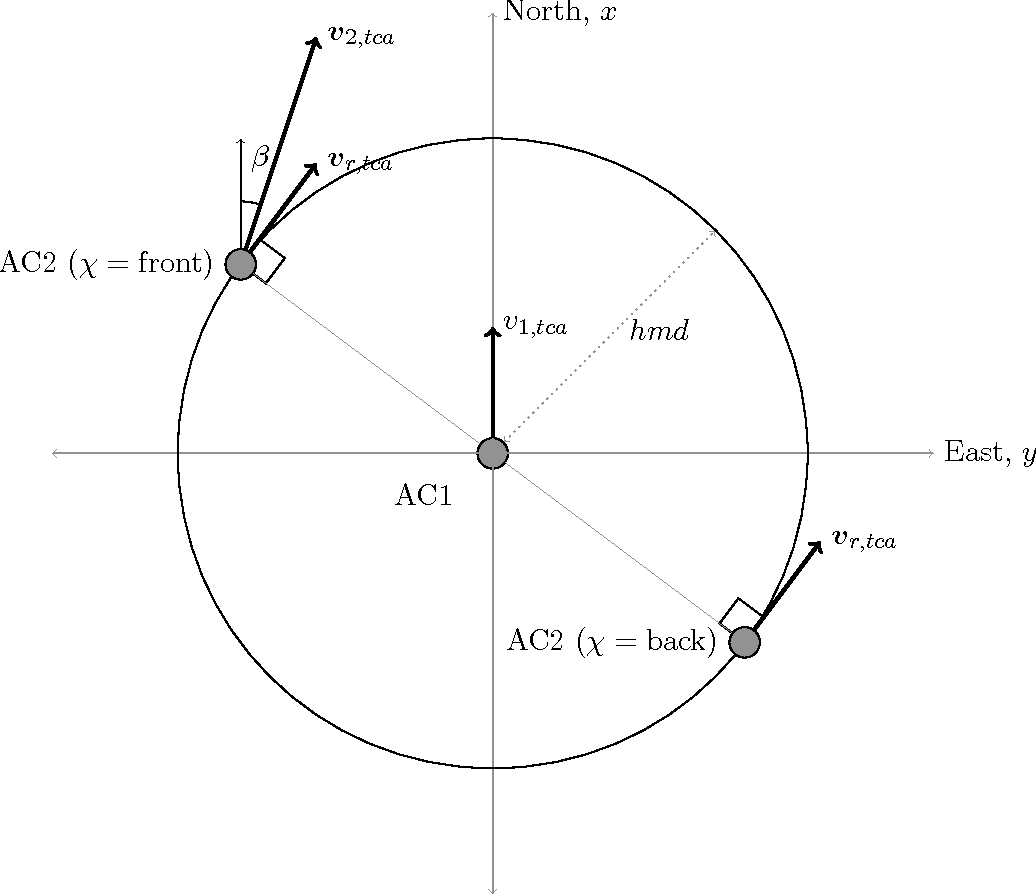
\includegraphics[width=\columnwidth]{encounter_geometry.png}
        \caption{Encounter geometry of 2 airplanes at their closest point of approach \cite{correnc}.}
        \label{fig:enc_geomt}
        \end{center}
    \end{figure}
    
\subsection{Outputs}
The \textit{TrainModel} method of our model uses state transition information to calculate a reward and stores it in the acas\_model.h5 file. Using this, the \textit{Predict(state)} method outputs one of 5 actions: \{$a_1, a_2, a_3, a_4, a_5$\} where $a_1$ and $a_2$ correspond to "Climb $h_{i} \leq h_{max}$ feet per minute" and "Descend $h_{i}\leq h_{max}$ feet per minute", respectively, while $a_3$ and $a_4$ correspond to "Turn left $\theta_{i}\leq\theta_{max}$ degrees" and "Turn right $\theta_{i} \leq \theta_{max}$ degrees", respectively. Here, $h_{max}$ and $\theta_{max}$ represent the maximum possible vertical velocity and turn rate for the specific aircraft. These are calculated by drawing conclusions from state information when practicable. $a_5$ corresponds to the action $COC$ or "Clear of Conflict". It describes a resolved encounter and allows ownship to move freely.  

\subsection{Reward}
Our neural network showed suboptimal performance with large rewards and penalties, leading us to surmise that the discontinuities in our initial rewards (+100 for an action resulting in a resolved NMAC, -100 for an encounter that ended in a NMAC, -10 for unnecessary maneuvers) produced significant loss terms. A review of \cite{deeprlcas} encouraged us to smooth the reward function with a sigmoid function. Additionally, we adjusted our rewards scale estimate to make the absolute maximum reward be -1. Reward is thus calculated using the following metrics:
\begin{itemize}
\item$R_1 = -(1 + e^{(r_{sep} - r_{min})/C})^{-1}$ where $hmd$ and $vmd$ work together to describe $r_{sep}$, the distance of separation while $r_{min}$ describes the minimum allowable separation (500 feet vertically and 200 feet horizontally\footnote{TCAS II thresholds often designate 500 feet of vertical and 100 feet horizontal separation as the minimum allowable separation. We chose 200 feet because it provides the pilot with more time to react, despite sacrificing potential resolutions to now untenable encounter scenarios.}) and $C$ is the smoothing applied to the step function.
\item$R_2 = -0.0002 \theta_{i}^2$ where $\theta_i$ represents the bank angle in degrees. This penalizes unnecessary maneuvering.
\item$R_3 = -0.04$ if $\theta_i \neq COC \lor h_i \neq COC$, penalizing false positives.
\item$R_4 = -0.0001 h_{i}$, penalizing unnecessary vertical movement.
\end{itemize}
The final reward is given by $R = R_1 + R_2 + R_3 + R_4$.

\subsection{Neural Network Implementation and Loss Function}
Our initial model used a 3-hidden-layer neural network with rectified linear activations between the hidden layers. ReLu was chosen in favor of other activation functions given its relative computational efficiency. We chose 3 hidden layers to speed up computation and avoid overfitting\footnote{Although we are now considering regularization as an alternative to reducing the number of layers.}. Instabilities inherent to reinforcement learning models using non-linear function approximators were well known and contained using the \textit{experience replay} mechanism explained in \cite{humanlevelcontrol}. We store the experiences $e_t = (s_t, a_t, r_t, s'_{t+1})$ at time-step t in memory. During the learning process, we apply Q-learning on batches of experiences sampled uniformly at random from the previously stored experiences to update the network parameters. A batch size of 128 was chosen with 84000 initial samples. Between batch update, we add 5 new samples while removing the oldest 5 samples from memory. This is to handle the limited capacity of our replay memory. Removing the oldest actions ensures that newer actions are sampled more than older actions. Given the stochastic nature of state transitions in a POMDP, we use the expectation of the next state and reward to describe our loss function \footnote{Such an expectation can be approximated by simulating several trajectories and averaging the Q values and rewards provided by the next states.} as follows: \[L(\theta) = \Bigg[\mathbb{E}(r + \gamma \: \underset{a' \in \overset{\circ}{A}}{max} \: Q(s', a', \theta^-)) - Q(s,a,\theta)\Bigg]^2 \]
It is worth noting that $\theta$ in the above function represents the neural network's parameters, not our turn rate input label.

\subsection{Algorithm}
The core algorithm is divided between the GDQNACAS algorithm\footnote{Generalized Deep Q Network Airborne Collision Avoidance System}, the methods controlling the Q functions, the set $D$ containing stored experiences, and the RLES simulator environment. The relationship between these components is described below:
\begin{algorithm}
\caption{Generalized DQN ACAS Algorithm}\label{dqnalg}
\begin{algorithmic}[1]
\State \textbf{Input:}
\State \qquad$Q$, class that contains the Q networks, implemented in file.jl
\State \qquad$D$, responsible for controlling experience replay
\State \qquad$S$, simulation environment
\Function{Begin:}{}
\While {not converged} 
\State$a \gets Q.obtainNextActionForState(s)$
\State $s', r \gets S.generateNewEncounterForState(s)$
\State $D.store(s,a,r,s')$ // Save agent experience.
\State$s \gets s'[0]$
\If{$hmd \geq 500$ or $vmd \geq 200$} 
\State $S.generateNewEncounterForState(s)$
\EndIf
\If{isTraining}
\State $batch \gets D.getSampleBatch()$
\State $Q.train(batch)$
\EndIf
\EndWhile
\State $Q.saveConvergedModel()$
\EndFunction
\end{algorithmic}
\end{algorithm}

\begin{algorithm}
\caption{Q Network Methods}\label{qnlbs}
\begin{algorithmic}[1]
\Function{obtainNextActionForState}{s}:
\State $incrementCounter()$
\If{$getCurrentCount() < initial\_size$}
\State \Return $rand(a) \mid rand(a) \in \overset{\circ}{A}$
\Else
\State $\epsilon \gets getEpsilonForCount(getCurrentCount())$
\If{$rand(0,1) < \epsilon$}
\State \Return $rand(a) \mid rand(a) \in \overset{\circ}{A}$
\Else
\State {\Return {$argmax(obtainRewardForState(s))$}}
\EndIf
\EndIf
\EndFunction
\end{algorithmic}
\end{algorithm}

\begin{algorithm}
\caption{Experience Memory D Methods}\label{dmethods}
\begin{algorithmic}[1]
\Function{getSampleBatch}{}
\For{$i \gets 0$}{ batch\_size}
\State\Return $rand(d) \mid d \in D$
\EndFor
\EndFunction
\end{algorithmic}
\end{algorithm}

\begin{algorithm}
\caption{Simulator Methods}\label{simmethods}
\begin{algorithmic}[1]
\Function{generateEncounterForState}{s}
\If{initial\_distribution}
\State \Return createSampleForDistribution(i)
\Else
\State \Return generateSampleFromEncounterModelWithFidelity(f)
\EndIf
\EndFunction

\Function{updateReceivedForSimulatorStateWithVector}{$u$}
\If{$u_{new} \mid u_{new} \not\in u_{initial}$ or altitudeInfoUpdated()}
\State $p \gets updatedPerformanceWithState(u)$
\State\Return{notifyPythonObserversWithUpdatedState(s)}
\EndIf
\EndFunction
\end{algorithmic}
\end{algorithm}
The Q network and D states are implemented in Python, while the simulator is written in Julia modules that readily interface with Python.

    % This is how you define a table: the [!hbt] means that LaTeX is forced (by the !) to place the table exactly here (by h), or if that doesnt work because of a pagebreak or so, it tries to place the table to the bottom of the page (by b) or the top (by t).
    \begin{table}[!hbt]
        % Center the table
        \begin{center}
        % Title of the table
        \caption{Simulation Parameters}
        \label{tab:simParameters}
        % Table itself: here we have two columns which are centered and have lines to the left, right and in the middle: |c|c|
        \begin{tabular}{|c|c|}
            % To create a horizontal line, type \hline
            \hline
            % To end a column type &
            % For a linebreak type \\
            Information message length & $k=16000$ bit \\
            \hline
            Radio segment size & $b=160$ bit \\
            \hline
            Rate of component codes & $R_{cc}=1/3$\\
            \hline
            Polynomial of component encoders & $[1 , 33/37 , 25/37]_8$\\
            \hline
        \end{tabular}
        \end{center}
    \end{table}

    % If you have questions about how to write mathematical formulas in LaTeX, please read a LaTeX book or the 'Not So Short Introduction to LaTeX': tobi.oetiker.ch/lshort/lshort.pdf

    % This is how you include a eps figure in your document. LaTeX only accepts EPS or TIFF files.
    \begin{figure}[!hbt]
        % Center the figure.
        \begin{center}
        % Include the eps file, scale it such that it's width equals the column width. You can also put width=8cm for example...
        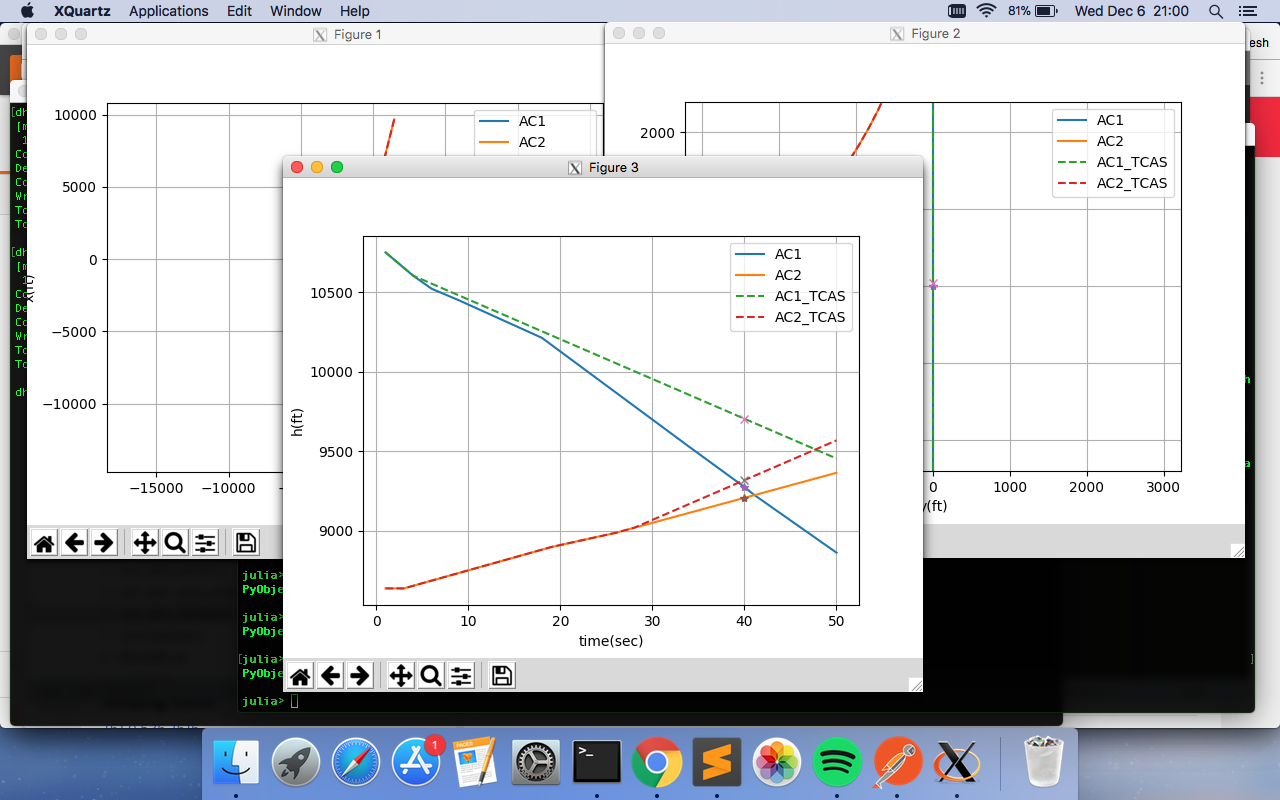
\includegraphics[width=\columnwidth]{tf_plot.png}
        % Create a subtitle for the figure.
        \caption{A trajectory plot. For Vincent: We will add in a more visible plot later.}
        % Define the label of the figure. It's good to use 'fig:title', so you know that the label belongs to a figure.
        \label{fig:tf_plot}
        \end{center}
    \end{figure}

\section{Evaluation}
Success is evaluated on the basis of two things:
\begin{itemize}
\item Risk Ratio and
\item Computational cost
\end{itemize}
We define the risk ratio as the ratio of the probability of a near mid-air collision occurring given the collision avoidance system's assistance divided by the nominal probability of a collision in the absence of using any collision avoidance system. A comparison charting TCAS' risk ratio against our algorithm's is available in figure 12. GDQNACAS easily outperforms TCAS in the 15000 scripted encounters we simulated. Yet, this is not conclusive evidence for GNQDCAS' safety. Monte Carlo Tree Searches can help maximize the likelihood of specific encounters designed to fail collision avoidance systems and would likely provide a higher quality estimate of both algorithms' respective safety margins. Despite the training step taking over 4 hours to develop on an early 2013 MacBook Pro, we are convinced that running our code on customized hardware would have provided quicker results. 
\\We also used the loss function as an effective signal to validate our approach. Unacceptable values output by the loss function in first iteration of our model made us research multiple causes\textemdash ranging from an error in the simulation framework, to model parameter considerations. Ultimately, redesigning the neural network to better approximate information entailed refining its reward component and using a different solver. We graph the differences between our initial loss function and its replacement in figure 13.

\section{Conclusion}
Our cursory investigation of this new approach to airborne collision avoidance gives us confidence that its potential benefits far outweigh its problems. While the system is admittedly averse to providing needless resolution advisories (given its reward function), adding more hidden layers would have likely helped us process state transitions better. 
\\The significant improvement in our system's risk ratio is the result of weeks of deliberation on possible viable solutions. We have all learned the importance of planning out an approach before investing time into implementing it. We hope other aviation and machine learning enthusiasts will use our model to build better, aircraft-agnostic collision avoidance systems.
\\The work done in this paper would not have been possible without the NAS correlated airspace encounter model, or the RLES software package,  both of which were designed by developed by Dr Mykel Kochenderfer at Stanford University. 

\section{Roles}
   % If you have questions about how to write mathematical formulas in LaTeX, please read a LaTeX book or the 'Not So Short Introduction to LaTeX': tobi.oetiker.ch/lshort/lshort.pdf
    % This is how you define a table: the [!hbt] means that LaTeX is forced (by the !) to place the table exactly here (by h), or if that doesnt work because of a pagebreak or so, it tries to place the table to the bottom of the page (by b) or the top (by t).
    \begin{table}[!hbt]
        % Center the table
        \begin{center}
        % Title of the table
        \caption{Team Member Roles}
        \label{tab:memberRoles}
        % Table itself: here we have two columns which are centered and have lines to the left, right and in the middle: |c|c|
        \begin{tabular}{|c|c|}
            % To create a horizontal line, type \hline
            \hline
            % To end a column type &
            % For a linebreak type \\
            \textbf{Task (approx. lines of code)} & \textbf{Lead} \\
            \hline\hline
            Connect the simulator to the neural network ($\sim 260$) & Dharmesh \\
            \hline
            Develop and tune neural network parameters ($\sim 200$) &Shantanu \& Kasim \\
            \hline
            Integrate adaptive stress testing framework into SISLES ($\sim 250)$ & Vincent\\
            \hline
        \end{tabular}
        \end{center}
    \end{table}

% Now we need a bibliography:
\begin{thebibliography}{5}

    %Each item starts with a \bibitem{reference} command and the details thereafter.
    \bibitem{tcaswhite}
    Munoz, C�sar, Anthony Narkawicz, and James Chamberlain. "A TCAS-II resolution advisory detection algorithm." Proceedings of the AIAA Guidance Navigation, and Control Conference and Exhibit. 2013.
    
    \bibitem{pomdporig}
    Temizer, Selim, et al. "Markov Decision Process Based Collision Avoidance Systems for Unmanned Aerial Vehicles."
    
    \bibitem{deeprlcas}
    Julian, Kyle D., and Mykel J. Kochenderfer. "Neural Network Guidance for UAVs." AIAA Guidance, Navigation, and Control Conference. 2017.
    
    \bibitem{googlego}
    Silver, David, et al. "Mastering the game of Go with deep neural networks and tree search." Nature 529.7587 (2016): 484-489.
APA

   \bibitem{kochbook}
   Kochenderfer, Mykel J. Decision making under uncertainty: theory and application. MIT press, 2015.
   
   \bibitem{sislcode}
   https://github.com/sisl/RLES-SISLES.jl "Sisl/RLES-SISLES.Jl." GitHub. N. p., 2017. Web. 13 Dec. 2017.
   
   \bibitem{tyronecite}
   https://github.com/puzzledsean/ACAS-542 "Harnessing Long Short Term Memory Networks for Aircraft Encounter Modeling" GitHub. N. p., 2017. Web. 13 Dec. 2017.
   
   \bibitem{correnc}
    Kochenderfer, M. J., et al. "Correlated encounter model for cooperative aircraft in the national airspace system version 1.0." Project Report ATC-344, Lincoln Laboratory (2008).
    
       \bibitem{correncmod}
    Kochenderfer, M. J., et al. "Correlated encounter model for cooperative aircraft in the national airspace system version 1.0." Project Report ATC-344, Lincoln Laboratory (2008).
    
    \bibitem{selfcode}
    https://github.com/weirdindiankid/cs542 "Weirdindiankid/Cs542." GitHub. N. p., 2017. Web. 13 Dec. 2017.
    
    \bibitem{humanlevelcontrol}
    Mnih, Volodymyr, et al. "Human-level control through deep reinforcement learning." Nature 518.7540 (2015): 529-533.
    
    \bibitem{nextgen}
    Billingsley, Thomas B., Mykel J. Kochenderfer, and James P. Chryssanthacopoulos. "Collision avoidance for general aviation." IEEE Aerospace and Electronic Systems Magazine 27.7 (2012): 4-12.
APA	

   \bibitem{pomdppolicexpansion}
   Ross, St�phane, et al. "Online planning algorithms for POMDPs." Journal of Artificial Intelligence Research 32 (2008): 663-704.
   
   \bibitem{cassattpap}
   Netjasov, Fedja, et al. "Development, validation and application of stochastically and dynamically coloured Petri net model of ACAS operations for safety assessment purposes." Transportation Research Part C: Emerging Technologies 33 (2013): 167-195.

    \bibitem{MJH06} % Conference paper
    T.~Mayer, H.~Jenkac, and J.~Hagenauer. Turbo base-station cooperation for intercell interference cancellation. {\em IEEE Int. Conf. Commun. (ICC)}, Istanbul, Turkey, pp.~356--361, June 2006.

    \bibitem{Proakis} % Book
    J.~G.~Proakis. {\em Digital Communications}. McGraw-Hill Book Co.,
    New York, USA, 3rd edition, 1995.

    \bibitem{talk} % Web document
    F.~R.~Kschischang. Giving a talk: Guidelines for the Preparation and Presentation of Technical Seminars.
    \url{http://www.comm.toronto.edu/frank/guide/guide.pdf}.

    \bibitem{5}
    IEEE Transactions \LaTeX and Microsoft Word Style Files.
    \url{http://www.ieee.org/web/publications/authors/transjnl/index.html}

\end{thebibliography}

% Your document ends here!
\end{document}